\chapter{Data Manipulation}

\section{Manipulating Geometrical Data}

There is a small number of function to manipulate geometric data in \ogs. The common approach to the manipulation of \ogs input data is that it should be changed in a GIS or other specialised software of the user's choice which usually offers much more functionality for these things than \ogs ever could.

Functions for the manipulation of geometric data that \emph{are} implemented are all associated with polylines and can be applied by right-clicking the ``Polylines'' item of any geometry and selecting \cmd{Connect Polylines...}.

\subsubsection{Connecting Polylines}
This function connects all the selected polylines to a single new polyline provided that the start- and end points of all segments are within the given maximum distance. The default maximum distance is $0.0$, meaning that start- and end points have to be identical.

Note that if more than two start/end points are located within the given maximum distance, still only two of those points are connected. These points are chosen randomly.

\subsubsection{Creating Polygons by Closing Polylines}
This function closes a (connected) polyline. Simply check `Close connected Polyline'. If a name has been entered, this name will be assigned to the closed polyline.

\subsubsection{Creating Surfaces by Triangulating Polygons}
This function additionally creates a new surface by triangulating the polygon. This simply requires checking `Create Surface from Polyline'. The newly created polyline has to be closed for that function to work. If a name has been entered, this name will be assigned to the surface.

\section{Creating Meshes from Geometry}

By selecting \cmd{Tools\ra Mesh Generation...} you open a dialog that allows you to create meshes using information currently present in the programme. For this to work you have to have GMSH\footnote{http://geuz.org/gmsh/} installed and be available from the location of the Data Explorer.

Specifically, you can select any geometry and observation sites that should be considered for generating the mesh. Note that all points of every data set considered for mesh generation will be included as nodes in the final mesh. Upon pressing \cmd{OK} a geometry-file for GMSH is written, GMSH is called to create the mesh and the newly created mesh is at once imported in the \ogs-Data Explorer.

There is an \cmd{Advanced}-Tab in this dialog that allows you set a number of parameters for the mesh. Most importantly you can select if you want an adaptive mesh or a homogeneous mesh. An adaptive mesh is refined towards points or lines specified in the geometry while a homogeneous mesh has elements of roughly the same size everywhere in the domain (see figure \ref{fig:meshing}).

\begin{figure}[tb]
\begin{center}
\subfloat[Geometry]{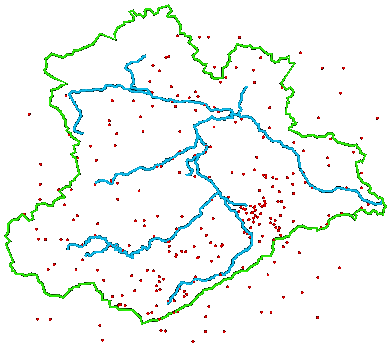
\includegraphics[width=0.3\linewidth]{meshing-geo}\label{meshing-geo}}\enspace
\subfloat[Homogeneous mesh]{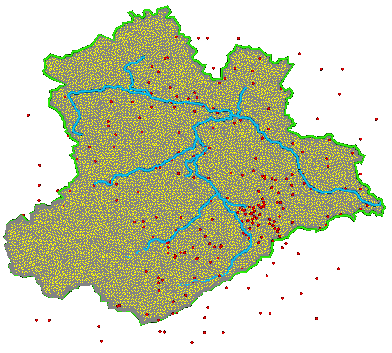
\includegraphics[width=0.3\linewidth]{meshing-hmg}\label{meshing-hmg}}\enspace
\subfloat[Adaptive mesh]{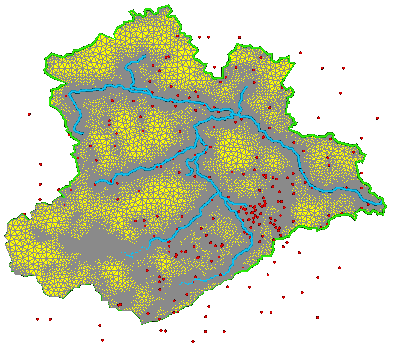
\includegraphics[width=0.3\linewidth]{meshing-adp}\label{meshing-adp}}
\end{center}
\caption{Meshing using geometric data and observation sites.} \label{fig:meshing}
\end{figure}

The specific parameters for adaptive meshes are:
\begin{itemize}
\item \textbf{Max. number of points in Quadtree leaf:} Generally speaking, the smaller this number the finer will the resulting mesh be. \\
    To be more exact, you have to have a basic idea what a quad tree \footnote{http://en.wikipedia.org/wiki/Quadtree} is. A tree structure is constructed by a sequential subdivision of the domain based on the distribution of relevant points in space. The criterium if a segment compromising a leaf is further refined is dependent on the number of points located in that segment. Therefore, larger numbers of that parameters will usually result in coarser meshes while smaller numbers will result in finer meshes. \emph{Note that this is technically not a correct explanation as results are heavily dependent on how many points are located in certain sub-divisions of the domain, the existence of point clusters, etc.}
\item \textbf{Mesh density scaling for points:} This is a scaling factor for the above parameter allowing for a refinement towards points located within the outer boundary. In general, smaller values will result in finer meshes.
\item \textbf{Mesh density scaling for stations:} This is exactly the same kind of scaling factor as for the option above, only for refinement towards observation sites.
\end{itemize}

Likewise, you can select an \textbf{Element Size} for homogeneous meshes. Here, too, a smaller number will result in a finer mesh.

\bigskip

Default parameters for all options are already predefined and have worked well with most examples that have been tested. Feel free to play around with these numbers but realise that the resulting mesh might not be what you have in mind.

\section{Extruding Meshes to 3D}

Any 2D mesh loaded into \ogs can be extruded into a 3D mesh by copying the 2D mesh layer a specified number of times and then connected any two neighbouring layers by creating 3D elements from all corresponding 2D elements (i.e. two triangles are connected and form one prism-elements, two quadrilateral elements form one hexahedron). This functionality can be accessed by right-clicking on a mesh in the data view and selecting \cmd{Edit Mesh...}. In the \cmd{3D Extrusion}-tab of the resulting dialog the number of mesh layers and the distance between neighbouring layers can be specified. 

For assigning elevation profiles to each layer, select the \cmd{Layer Mapping}-tab. Here, for each layer of the mesh a raster file in *.asc format can be selected and will be assigned to the respective mesh layer. 
\emph{Note that currently the check if two layers are intersecting each other does \emph{not} work correctly!}

\section{Analyse Mesh Quality}

You can visualise the quality of a given mesh by right-clicking on the mesh in the respective data view and selecting \cmd{Check Mesh Quality...}. This allows to choose between currently four implemented measurements for mesh element quality. The result of choosing any of these modes is a colour-codes overlay of the mesh where every element is assigned a quality in $[0,1]$. You can select this overlay in the visualisation pipeline and specify thresholds to select a certain range of quality and see which element fall into that range. \emph{(Note: You might need to manually set the correct scalar array for visualising mesh quality. The appropriate data can be chosen by selecting in ``C-Selection'' in the \cmd{Active Scalar} pull-down menu.}

\begin{figure}[tb]
\begin{center}
\subfloat[Edge Aspect Ratio]{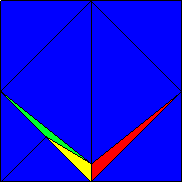
\includegraphics[width=0.3\linewidth]{MshQualEdgeRatio}\label{fig:mshqual1}}\enspace
\subfloat[Element Area]{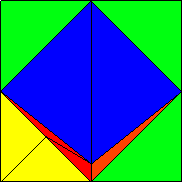
\includegraphics[width=0.3\linewidth]{MshQualArea}\label{fig:mshqual2}}\enspace
\subfloat[EquiAngle Skewness]{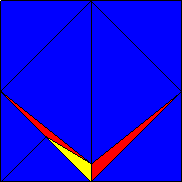
\includegraphics[width=0.3\linewidth]{MshQualEquiAngle}\label{fig:mshqual3}}
\end{center}
\caption{Examples for colour coded mesh quality measurements.} \label{fig:mshqual}
\end{figure}

The currently implemented measures are the following:
\begin{itemize}
\item \textbf{Aspect Ratio of Edge Length:} Analyses the ratio of shortest to longest edge of every element. Equilateral elements are often considered superior and better suited for FEM simulation, therefore these elements are rated ``1'' with their quality degrading with increasing differences in edge length. Each element is assigned the value of the highest ratio between any two of its edges. This is a good measure for triangle elements but might be not as good as others. See figure \ref{fig:mshqual1}.
\item \textbf{Area of 2D Elements:} Compares the area of all 2D elements (this includes the faces of 3D elements!) by assigned ``1'' to the element with the largest area and ``0'' to the element with the smallest area. See figure \ref{fig:mshqual2}.
\item \textbf{Volume of 3D Elements:} As with the area-criterion, this measure compares the volume of 3D mesh elements. 2D elements are ignored when this option is selected.
\item \textbf{Angles between Adjacent Edges:} Calculates the maximum deviation of an angle between any two adjacent edges of the element from the ``optimum'' angle, i.e. the angle of an equiangular element. This optimum angle is $90\degree$ for triangles or tetrahedra and $90\degree$ for quadrilateral or hexahedral elements. This measurement is called \emph{EquiAngle Skewness} and given by
    \begin{equation}
    s = \max\left[\frac{\theta_{max}-\theta_{opt}}{180-\theta_{opt}},\frac{\theta_{opt}-\theta_{min}}{\theta_{opt}}\right]
    \end{equation}
    where $\theta_{max}$ is the maximum angle between any two edges found in the element, $\theta_{min}$ is the minimum angle and $\theta_{opt}$ is the optimum angle.
    See figure \ref{fig:mshqual3}.
\end{itemize}

The quality measure best suited for a given mesh might depend on the process you want to simulate using this mesh. For instance, processes such as groundwater recharge consist mainly of layered flows, meaning that large differences between horizontal and vertical element surfaces might have no effect on a correct result. The simulation of mass transport processes explicitly requires a fine mesh resolution in vertical direction to ensure a stable solution.

\section{Time series data and stratigraphic data}

For observation sites it is possible to display additional information such as logger data at the site or the stratigraphy at a borehole. Both features are currently only implemented as a proof of concept and need to be expanded in the future.

To view the additional information of an observation site load a stn-file into the programm and right-click on any observation site in the data view. You will see either the menu entry ``View Stratigraphy...'' for a borehole or ``View Diagram...'' for a station. If you selected to view a diagram, a dialog will open which allows you to select a start and end date or to load a file that contains the data (if no associated data base entry for the station has been found). A new window will open, displaying the requested information.

